\documentclass[12pt]{article}
\usepackage{amsfonts, amssymb, amsmath, amsthm}
\usepackage[margin=1in]{geometry}
\usepackage{tikz}
\usetikzlibrary{patterns, decorations.pathreplacing, arrows.meta}

\pagestyle{myheadings}
\markright{Explainer: Rudin 4.3 --- Zero Sets are Closed\hfill}

\newcommand{\R}{\mathbb{R}}

\begin{document}

\begin{center}
    \textbf{\Large Zero Sets of Continuous Functions are Closed}\\[0.5em]
    \large A visual guide to Rudin 4.3
\end{center}

\section{What is a Zero Set?}

Given a continuous function $f : X \to \R$, the \textbf{zero set} is:
\[
Z(f) = \{p \in X : f(p) = 0\} = f^{-1}(\{0\})
\]

It's simply the set of points where $f$ equals zero.

\begin{center}
\begin{tikzpicture}[scale=0.9]
    \draw[->] (-4, 0) -- (4, 0) node[right] {$x$};
    \draw[->] (0, -1.5) -- (0, 2.5) node[above] {$y$};

    % A continuous function that crosses zero
    \draw[blue, thick, domain=-3.5:3.5, samples=100]
        plot (\x, {0.3*(\x+2)*(\x)*(\x-2.5)});

    \node[blue] at (3, 2) {$y = f(x)$};

    % Mark zeros
    \fill[red] (-2, 0) circle (3pt);
    \fill[red] (0, 0) circle (3pt);
    \fill[red] (2.5, 0) circle (3pt);

    \node[red] at (-2, -0.5) {$p_1$};
    \node[red] at (0, -0.5) {$p_2$};
    \node[red] at (2.5, -0.5) {$p_3$};

    \node[red, text width=4cm, align=center] at (-2, -1.5) {$Z(f) = \{p_1, p_2, p_3\}$};
\end{tikzpicture}
\end{center}

\section{What Does ``Closed'' Mean Again?}

A set is \textbf{closed} if its complement is open.

Equivalently: a set is closed if it contains all its limit points.

\begin{center}
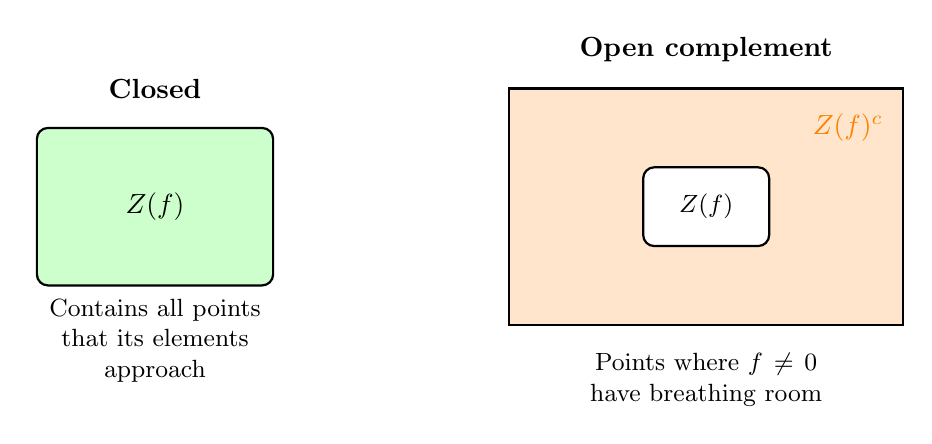
\begin{tikzpicture}[scale=1]
    % Closed set
    \begin{scope}[xshift=-3.5cm]
        \draw[thick, rounded corners, fill=green!20] (-1.5, -1) rectangle (1.5, 1);
        \node at (0, 0) {$Z(f)$};
        \node at (0, 1.5) {\textbf{Closed}};
        \node[font=\small, text width=3cm, align=center] at (0, -1.7) {Contains all points\\that its elements\\approach};
    \end{scope}

    % Open complement
    \begin{scope}[xshift=3.5cm]
        \draw[thick, fill=orange!20] (-2.5, -1.5) rectangle (2.5, 1.5);
        \draw[thick, rounded corners, fill=white] (-0.8, -0.5) rectangle (0.8, 0.5);
        \node at (0, 0) {\small $Z(f)$};
        \node[orange] at (1.8, 1) {$Z(f)^c$};
        \node at (0, 2) {\textbf{Open complement}};
        \node[font=\small, text width=3.5cm, align=center] at (0, -2.2) {Points where $f \neq 0$\\have breathing room};
    \end{scope}
\end{tikzpicture}
\end{center}

\section{The Intuition: Why is $Z(f)$ Closed?}

If $f$ is continuous and $f(p) \neq 0$, then $f$ is ``stuck away from zero'' near $p$.

\begin{center}
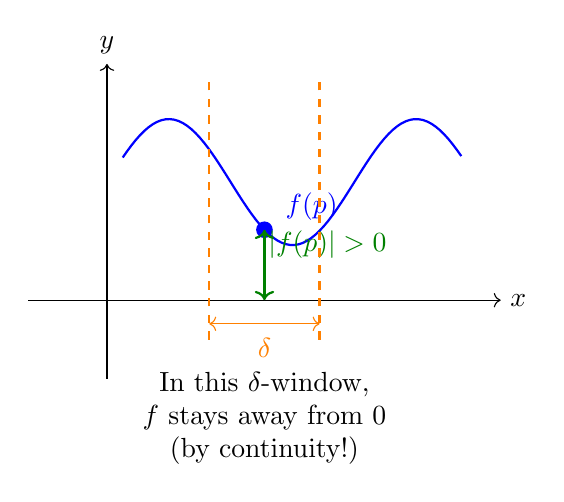
\begin{tikzpicture}[scale=1]
    \draw[->] (-1, 0) -- (5, 0) node[right] {$x$};
    \draw[->] (0, -1) -- (0, 3) node[above] {$y$};

    % Function
    \draw[blue, thick, domain=0.2:4.5, samples=80] plot (\x, {1.5 + 0.8*sin(2*\x r)});

    % Point p where f(p) != 0
    \fill[blue] (2, {1.5 + 0.8*sin(4 r)}) circle (3pt);
    \node[blue] at (2.6, {1.8 + 0.8*sin(4 r)}) {$f(p)$};

    % Show |f(p)| > 0
    \draw[<->, green!50!black, thick] (2, 0) -- (2, {1.5 + 0.8*sin(4 r)});
    \node[green!50!black] at (2.8, 0.7) {$|f(p)| > 0$};

    % Delta neighborhood
    \draw[orange, thick, dashed] (1.3, -0.5) -- (1.3, 2.8);
    \draw[orange, thick, dashed] (2.7, -0.5) -- (2.7, 2.8);
    \draw[<->, orange] (1.3, -0.3) -- (2.7, -0.3);
    \node[orange] at (2, -0.6) {$\delta$};

    \node[text width=5cm, align=center] at (2, -1.5) {In this $\delta$-window,\\$f$ stays away from $0$\\(by continuity!)};
\end{tikzpicture}
\end{center}

\textbf{Key insight:} Continuity means $f$ can't ``jump.'' If $f(p)$ is some distance from $0$, then nearby values of $f$ are also bounded away from $0$.

\section{The Proof Strategy}

We show $Z(f)^c = \{p : f(p) \neq 0\}$ is open.

\begin{center}
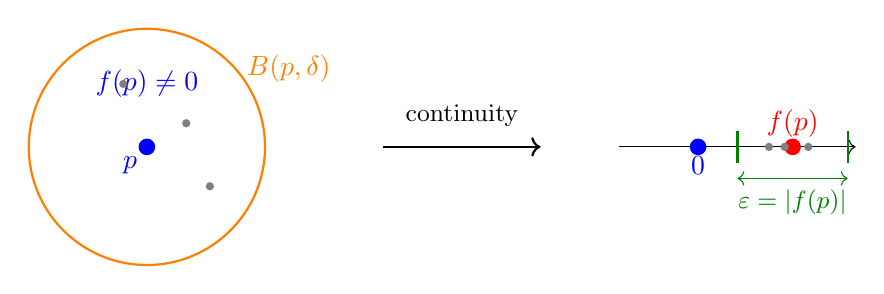
\begin{tikzpicture}[scale=1]
    % Point p not in Z(f)
    \fill[blue] (0, 0) circle (3pt) node[below left] {$p$};
    \node[blue] at (0, 0.8) {$f(p) \neq 0$};

    % Delta ball
    \draw[orange, thick] (0, 0) circle (1.5);
    \node[orange] at (1.8, 1) {$B(p, \delta)$};

    % Points inside
    \fill[gray] (0.5, 0.3) circle (1.5pt);
    \fill[gray] (-0.3, 0.8) circle (1.5pt);
    \fill[gray] (0.8, -0.5) circle (1.5pt);

    \draw[->, thick] (3, 0) -- (5, 0);
    \node at (4, 0.4) {\small continuity};

    % After applying f
    \begin{scope}[xshift=7cm]
        \draw[->] (-1, 0) -- (2, 0);
        \fill[blue] (0, 0) circle (3pt) node[below] {$0$};

        % f(p) away from 0
        \fill[red] (1.2, 0) circle (3pt) node[above] {$f(p)$};

        % epsilon neighborhood
        \draw[green!50!black, thick] (0.5, -0.2) -- (0.5, 0.2);
        \draw[green!50!black, thick] (1.9, -0.2) -- (1.9, 0.2);
        \draw[<->, green!50!black] (0.5, -0.4) -- (1.9, -0.4);
        \node[green!50!black, font=\small] at (1.2, -0.7) {$\varepsilon = |f(p)|$};

        % All nearby values stay away from 0
        \fill[gray] (0.9, 0) circle (1.5pt);
        \fill[gray] (1.4, 0) circle (1.5pt);
        \fill[gray] (1.1, 0) circle (1.5pt);
    \end{scope}
\end{tikzpicture}
\end{center}

\textbf{The argument:}
\begin{enumerate}
    \item Let $p \notin Z(f)$, so $|f(p)| > 0$
    \item Set $\varepsilon = |f(p)|$
    \item By continuity: there exists $\delta > 0$ such that $|f(x) - f(p)| < \varepsilon$ when $d(x,p) < \delta$
    \item Triangle inequality: $|f(x)| \geq |f(p)| - |f(x) - f(p)| > \varepsilon - \varepsilon = 0$
    \item So $f(x) \neq 0$ for all $x$ near $p$ --- meaning $B(p, \delta) \subset Z(f)^c$
\end{enumerate}

\section{The Triangle Inequality Trick}

This is a standard technique worth remembering:

\begin{center}
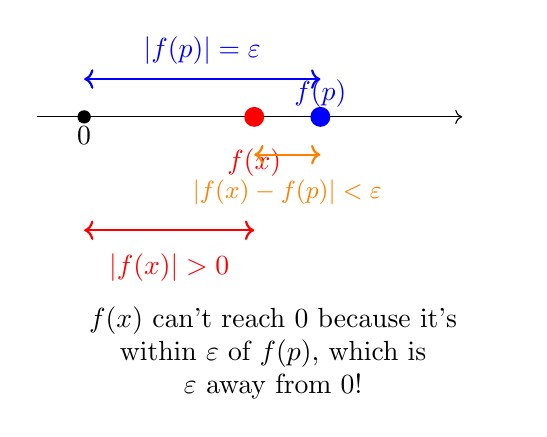
\begin{tikzpicture}[scale=1.2]
    \draw[->] (-0.5, 0) -- (4, 0);

    \fill (0, 0) circle (2pt) node[below] {$0$};
    \fill[blue] (2.5, 0) circle (3pt) node[above] {$f(p)$};
    \fill[red] (1.8, 0) circle (3pt) node[below=8pt] {$f(x)$};

    % |f(p)|
    \draw[blue, thick, <->] (0, 0.4) -- (2.5, 0.4);
    \node[blue] at (1.25, 0.7) {$|f(p)| = \varepsilon$};

    % |f(x) - f(p)|
    \draw[orange, thick, <->] (1.8, -0.4) -- (2.5, -0.4);
    \node[orange, font=\small] at (2.15, -0.8) {$|f(x) - f(p)| < \varepsilon$};

    % |f(x)|
    \draw[red, thick, <->] (0, -1.2) -- (1.8, -1.2);
    \node[red] at (0.9, -1.6) {$|f(x)| > 0$};

    \node[text width=6cm, align=center] at (2, -2.5) {$f(x)$ can't reach $0$ because it's\\within $\varepsilon$ of $f(p)$, which is\\$\varepsilon$ away from $0$!};
\end{tikzpicture}
\end{center}

\section{Alternative Viewpoint: Preimages}

There's an even slicker way to see this:
\begin{itemize}
    \item $Z(f) = f^{-1}(\{0\})$
    \item $\{0\}$ is a closed subset of $\R$
    \item Continuous functions pull back closed sets to closed sets
    \item Therefore $Z(f)$ is closed!
\end{itemize}

Both approaches work. The $\varepsilon$-$\delta$ proof is more hands-on; the preimage proof is more conceptual.

\end{document}
